\chapter{Contesto aziendale}

\section{Dominio applicativo}
% Breve introduzione al settore del \textit{Enterprise Application Integration}, al tipo di clientela (ovvero pubblica e privata di grandi dimensioni, big data), alla tipologia di \textit{software} prodotti dall’azienda per la clientela (\textit{Middleware}), e alla propensione all’innovazione (richieste da parte della clientela
In conclusione al percorso di studi del corso di laurea in Informatica ho effettuato lo \textit{stage} presso \textit{Sync Lab}.
Questa è un'azienda di produzione software e integrazione di sistemi che fornisce principalmente prodotti per clienti di grande dimensione, sia pubblici che privati.

L'azienda è suddivisa in diversi settori con diverse sedi; l'esperienza personale mi ha portato a conoscere il settore dell'\textit{Enterprise Architecture Integration} e del \textit{Tecnical Professional Services Padova} nella sede aziendale di Padova.
Il percorso di \textit{stage} che ho intrapreso è associato al primo di questi, che si occupa principalmente dell'EAI (\textit{Enterprise Application Integration}) ovvero dell'integrazione funzionale di applicazioni aziendali per una clientela di grandi dimensioni, tramite sistemi di integrazione \textit{Middleware}.

I \textit{Middleware} prodotti comprendono l'utilizzo di molteplici linguaggi e tecnologie in continua evoluzione; è un contesto con un'importante propensione all'innovazione, talvolta esplicitamente richiesta dai clienti.

\section{Processi interni e strumenti organizzativi}

% Esposizione delle norme organizzative (\textit{online meeting}, \textit{smart working}, presenze in sede), degli strumenti utilizzati nel rapporto con l’azienda (chat, email e \textit{Project Board}), e delle norme di progetto.
%
% \bigskip\noindent
% Processi interni in cui sono stato coinvolto: Sviluppo, Collaudo, Verifica, Formazione, Manutenzione/Evoluzione.

% \bigskip\noindent
% Breve presentazione dei ruoli delle persone coinvolte nel percorso di \textit{stage}.

L'azienda adotta dei processi interni per delineare l'avanzamento di un progetto.
Durante il percorso di \textit{stage} sono stato coinvolto nei processi di Formazione, Sviluppo, Verifica e Collaudo; i processi di Manutenzione ed Evoluzione sono stati solamente accennati in quanto al di fuori dello scopo del percorso.
Questi processi, nella mia esperienza personale, non sono stati delineati rigorosamente, al fine di garantire una certa rapidità e adattabilità al progetto di sperimentazione.
Ogni processo è suddiviso in attività modulari, per rendere l'avanzamento efficace e quantificabile.

L'organizzazione efficiente di un progetto è garantita dal corretto utilizzo dei vari strumenti a supporto quali \textit{Kanban Board} (come \textit{Click Up} per la gestione di progetto e \textit{Notion} per le prenotazioni della postazione di lavoro in sede), \textit{chat} (come \textit{Google Chat}) per i confronti rapidi con gli altri membri interni al progetto, ed e-mail per le comunicazioni con componenti esterni al progetto.

\begin{figure}[h]
  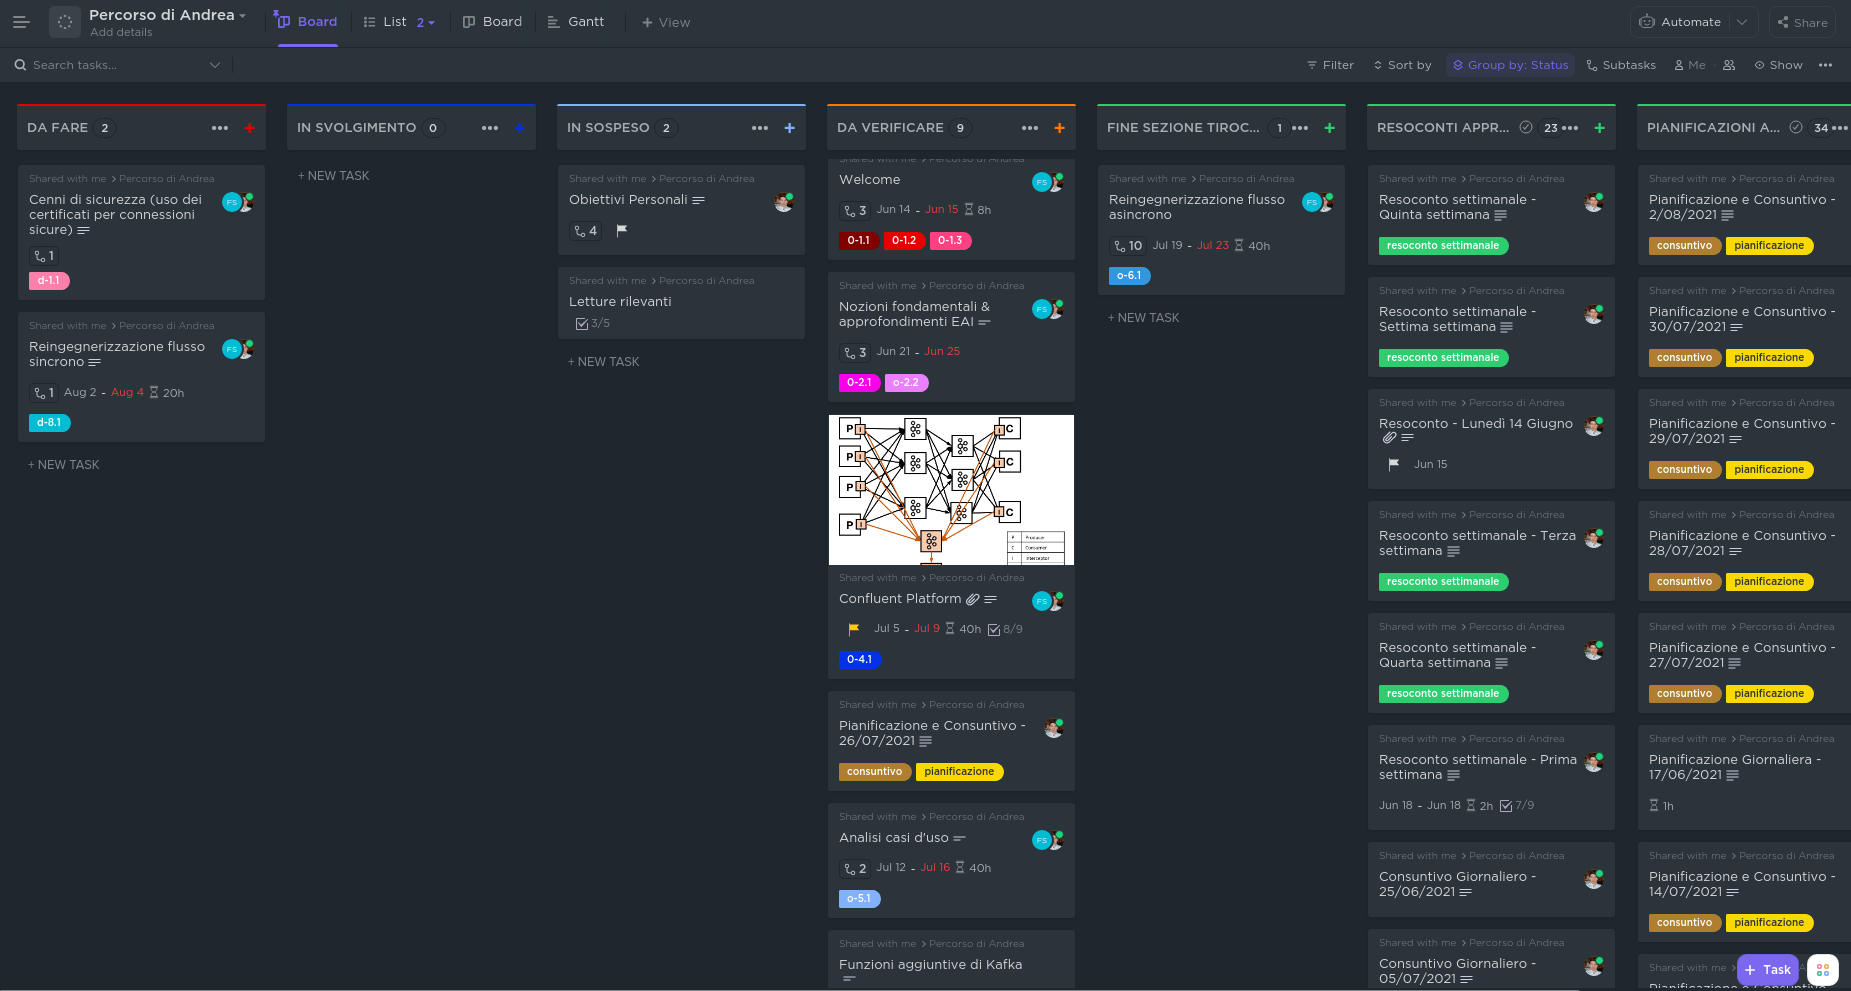
\includegraphics[width=\textwidth]{images/clickup_board.png}\\
  \caption{\textit{Kanban Board} del progetto di \textit{stage}}
\end{figure}
\begin{figure}[h!]
  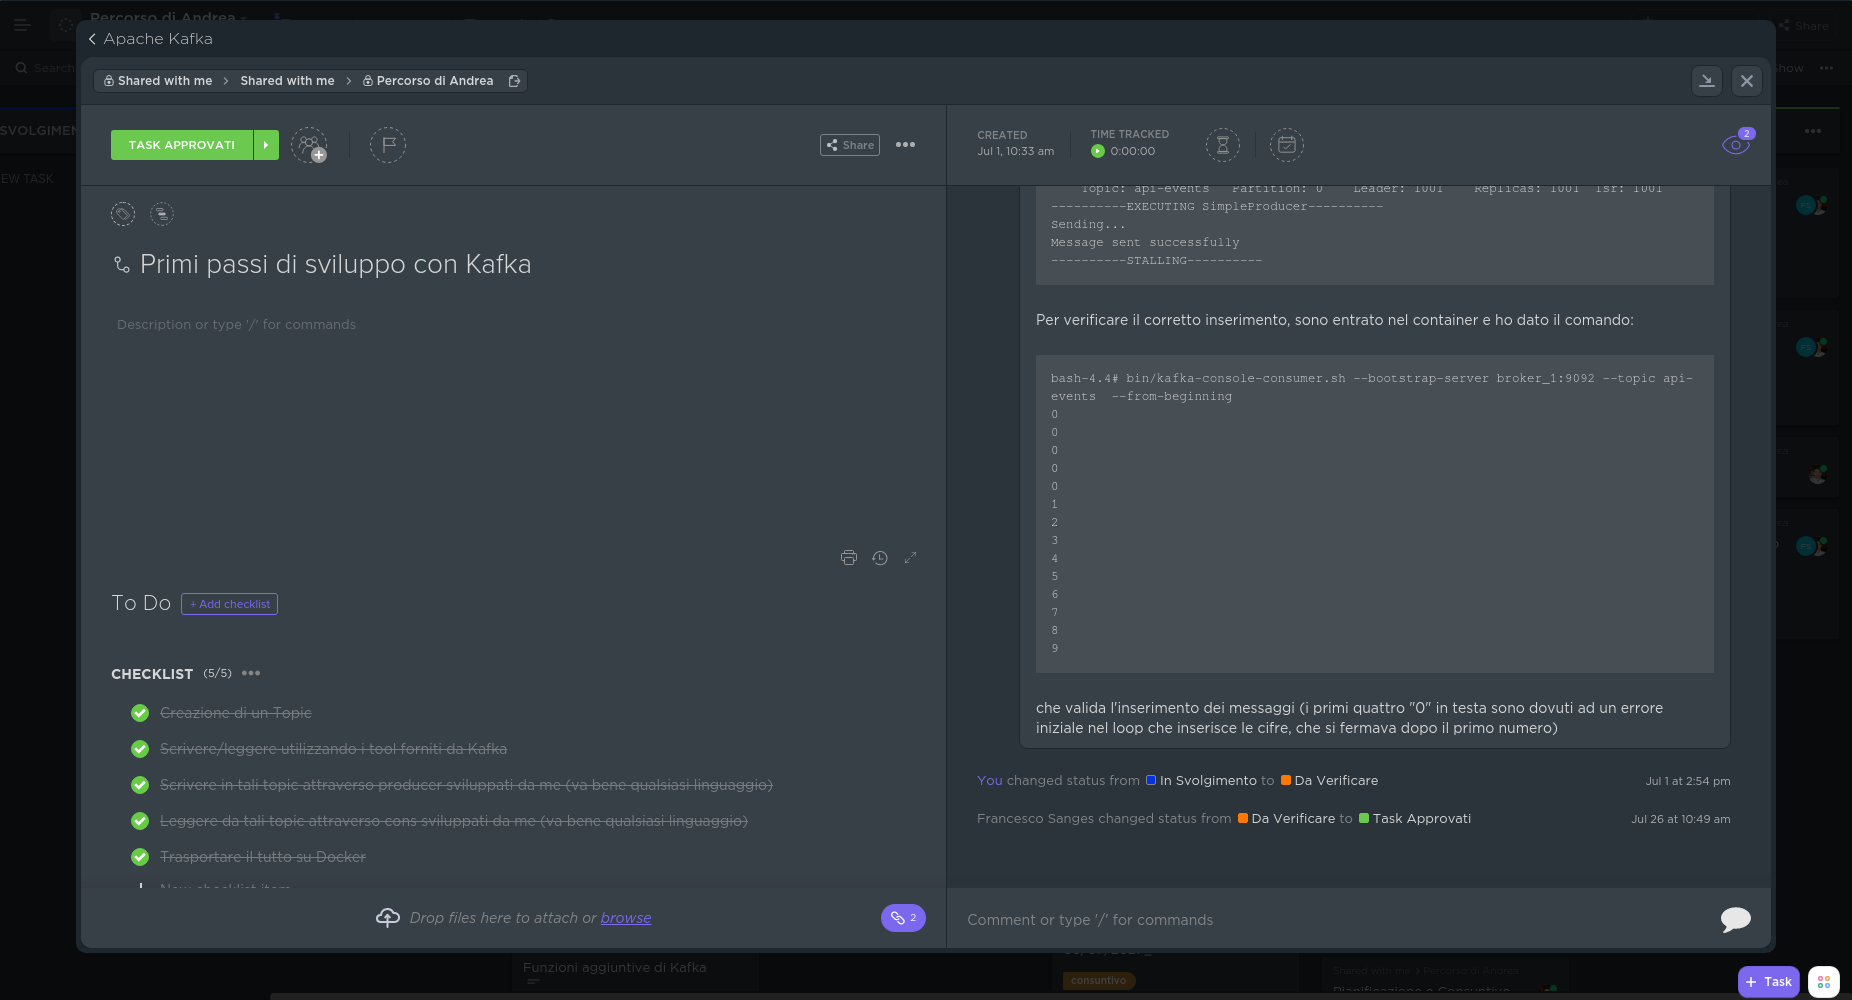
\includegraphics[width=\textwidth]{images/clickup_task.png}\\
  \caption{Esempio di un'attività del processo di Formazione}
\end{figure}

\section{L’ambiente di lavoro}

% Sviluppo indipendente dal sistema operativo, produzione di \textit{software} non strettamente legati ad uno specifico linguaggio, utilizzo di ambienti virtuali quali \textit{Virtual Machine} e \textit{container} per simulare sistemi indipendenti.
L'ambiente di lavoro di cui ho avuto esperienza risulta abbastanza libero e flessibile.
Lo sviluppo del prodotto nell'ambito del EAI dev'essere indipendente dal linguaggio di programmazione, dagli strumenti utilizzati per l'esecuzione e sviluppo, e possibilmente anche dal Sistema operativo su cui eseguire il \textit{software}.
A tal scopo si utilizzano strumenti quali \textit{Virtual Machine} e \textit{Container}: essi non sono garantiscono l'indipendenza dal Sistema Operativo in uso, ma simulano efficacemente il caso d'uso reale in cui i vari eseguibili sono dislocati in più computer o server come spesso accade per il cliente.
Nonostante il percorso formativo abbia visto l'apprendimento di entrambe le tecnologie tramite l'utilizzo dei software \textit{Virtual Box} e \textit{Docker}, infine solo quest'ultima è stata utilizzata durante il progetto poichè più efficente e minimale.
